% -*- flyspell-dict: "german" -*-

\documentclass[xcolor=dvipsnames]{beamer}
\mode<presentation>{
  \usetheme{main}
}

\usepackage[ngerman]{babel}
\usepackage[utf8x]{inputenc}
\usepackage{times}
\usepackage[T1]{fontenc}
\usepackage{textcomp}
\usepackage{graphicx}
\usepackage{listings}
\usepackage{semantic}
\usepackage{multicol}
\usepackage{hyperref}
\reservestyle{\command}{\textbf}
\command{accept, request, in}
\bibliographystyle{alphadin}

% ----------------------------------------------------------
% title page:

\title{Infrastrukturkosten Stadt- und Straßenbahnen}

\author[Brandes, Müller, Riecken, Sigler, Sulfrian (Gruppe 7)]{Yves~Müller \and
  Marian~Sigler \and
  Alexander~Sulfrian \and
  Dario~Lino~Brandes \and
  Robert~Hanns~Riecken}
\institute{\\ \vspace{1em}
  Institut für Land- und Seeverkehr\\
  Fachgebiet Schienenfahrwege und Bahnbetrieb\\
  Technische Universität Berlin}

\day=28 \month=05 \year=2013
\date{\today}

% ----------------------------------------------------------

\begin{document}

% ----------------------------------------------------------

\begin{frame}
  \titlepage
\end{frame}

% ----------------------------------------------------------

\begin{frame}
  \frametitle{Inhalt}

  \setcounter{tocdepth}{2}
  \tableofcontents
\end{frame}

% ----------------------------------------------------------

\section{Definitionen}
\begin{frame}
  \frametitle{Definitionen}

  \begin{itemize}
  \item nur Bahnen nach BOStrab
  \item Kategorisierung:
    \begin{itemize}
    \item U-Bahn bzw. Hochbahn
    \item Straßenbahn
    \end{itemize}
  \item Differenzierung von Streckenabschnitten in Tunnel
    oder auf Brücken
  \end{itemize}
\end{frame}

% ----------------------------------------------------------

\section{Vorgehen}
\begin{frame}
  \frametitle{Vorgehen}

  \begin{itemize}
  \item Ermittlung Daten für div. Projekte:
    \begin{itemize}
    \item geplante/tatsächliche Kosten
    \item Strecken-/Gleislänge
    \item Anzahl Ausweichstellen/Haltstellen
    \item Tunnel-/Brücken- und Hochbahnanteil
    \item und weitere
    \end{itemize}
  \item Umrechnung und Inflationsbereinigung
  \item Berechnung von Durchschnittskosten
  \end{itemize}
\end{frame}


\section{Vorstellung ausgewählter Strecken}
% ----------------------------------------------------------

\subsection{Darmstadt}
\begin{frame}
  \frametitle{Darmstadt (1897)}

  \begin{itemize}
  \item Länge: 6,4km eingleisig mit 8 Ausweichen
    \begin{itemize}
    \item 5,5 km eingleisig
    \item 8 Ausweichen
    \item 0,9 km zweigleisig
    \end{itemize}
  \item Baukosten: 287.000 Mark (5,1 Mio. €)
    \begin{itemize}
    \item Preis pro km: 0,7 Mio. €/km\\
      (2-gleisige Abschnitte doppelt gewichtet)
    \end{itemize}
  \end{itemize}
\end{frame}

% ----------------------------------------------------------

\begin{frame}
  \frametitle{Darmstadt (1899 bis 1903)}

  \begin{itemize}
  \item Diverse Neubaustrecken, Gesamtlänge: 5,98 km
    \begin{itemize}
    \item 5,34 km eingleisig
    \item 4 Ausweichen
    \item 0,64 km zweigleisig
    \end{itemize}
  \item Gesamtkosten: 1,2 Mio. Mark (inklusive Fahrzeuge; etwa 50\%
    davon für Gleisbau)
    \begin{itemize}
    \item Umgerechnet ca. 5,6 Mio. €
    \item Preis pro km: 0,85 Mio. €/km (0,09 Mio. Mark/km)\\
      (2-gleisige Abschnitte doppelt gewichtet)
    \end{itemize}
  \end{itemize}
\end{frame}

% ----------------------------------------------------------

\subsection{Bergen}
\begin{frame}
  \frametitle{Bergen (2010)}

  \begin{itemize}
  \item Länge: 9,8 km
    \begin{itemize}
    \item 4 Tunnel (2,63 km)
    \item Gesamte Strecke 2-gleisig
    \end{itemize}
  \item Baukosten:
    \begin{itemize}
    \item Insgesamt: 140 Mio. € (projektiert, abzgl. ca. 30
      Mio. € für Fahrzeuge)
    \item Preis pro km: 11,2 Mio. €/km
    \end{itemize}
  \item zwei weitere Ausbaustufen geplant
  \end{itemize}
\end{frame}

% ----------------------------------------------------------

\subsection{Aarhus}
\begin{frame}
  \frametitle{Aarhus (2016)}

  \begin{itemize}
  \item Länge:
    \begin{itemize}
    \item Gesamtlänge: 12,0 km
    \item Keine Tunnelneubauten
    \item Weitestgehend auf vorhanden Eisenbahntrassen
    \end{itemize}
  \item Baukosten:
    \begin{itemize}
    \item Insgesamt: 500 Mio. Kronen
    \item Umgerechnet 65 Mio. € (0,13 €/Krone)
    \item Preis pro km: 5,4 Mio. €/km
    \end{itemize}
  \end{itemize}
\end{frame}

% ----------------------------------------------------------

\subsection{Stuttgart}
\begin{frame}
  \frametitle{Stuttgart-Stammheim (2011)}

  \begin{itemize}
  \item Länge: 2,985 km
    \begin{itemize}
    \item ein Tunnel (1 km)
    \item 7 Haltestellen
    \item ersetzt Straßenbahn
    \end{itemize}
  \item Baukosten: 105 Mio. €
    \begin{itemize}
    \item 35,2 Mio. €/km
    \end{itemize}
  \end{itemize}
\end{frame}

% ----------------------------------------------------------

\subsection{Toulouse}
\begin{frame}
  \frametitle{Straßenbahn Toulouse (2010)}

  \begin{itemize}
  \item Länge: 11 km
    \begin{itemize}
    \item 18 Haltestellen
    \item überirdisch, eine Brücke
    \end{itemize}
  \item Baukosten: 212 Mio. €
    \begin{itemize}
    \item 19,3 Mio. €/km
    \end{itemize}
  \end{itemize}
\end{frame}

% ----------------------------------------------------------

\subsection{Magdeburg}
\begin{frame}
  \frametitle{Magdeburg}

  \begin{itemize}
  \item Straßenbahnstrecke nach Reform
  \item dritter Bauabschnitt einer neuen Nord-Süd-Verbindung
  \item Länge: 3.6km
    \begin{itemize}
    \item 8 Haltestellen
    \item komplette Strecke 2-gleisig
    \item etwa 500m: auf der Straße, Rest: eigener Gleiskörper
    \end{itemize}
  \item Baukosten: 22 Mio. €
    \begin{itemize}
    \item 6,1 Mio. €/km
    \end{itemize}
  \end{itemize}
\end{frame}

% ----------------------------------------------------------

\subsection{Dubai}
\begin{frame}
  \frametitle{Dubai}

  \begin{itemize}
  \item U-Bahn Neubau (seit 2005)
  \item Länge: 74km
    \begin{itemize}
    \item 47 Stationen
    \item 12km unterirdisch, Rest als Hochbahn
    \item fahrerlos
    \item Bahnhöfe klimatisiert
    \end{itemize}
  \item Baukosten: 5,7 Mrd. €
    \begin{itemize}
    \item 77 Mio. €/km
    \end{itemize}
  \end{itemize}
\end{frame}

% ----------------------------------------------------------

\section{Erste Ergebnisse}
\begin{frame}
  \frametitle{Erste Ergebnisse}
  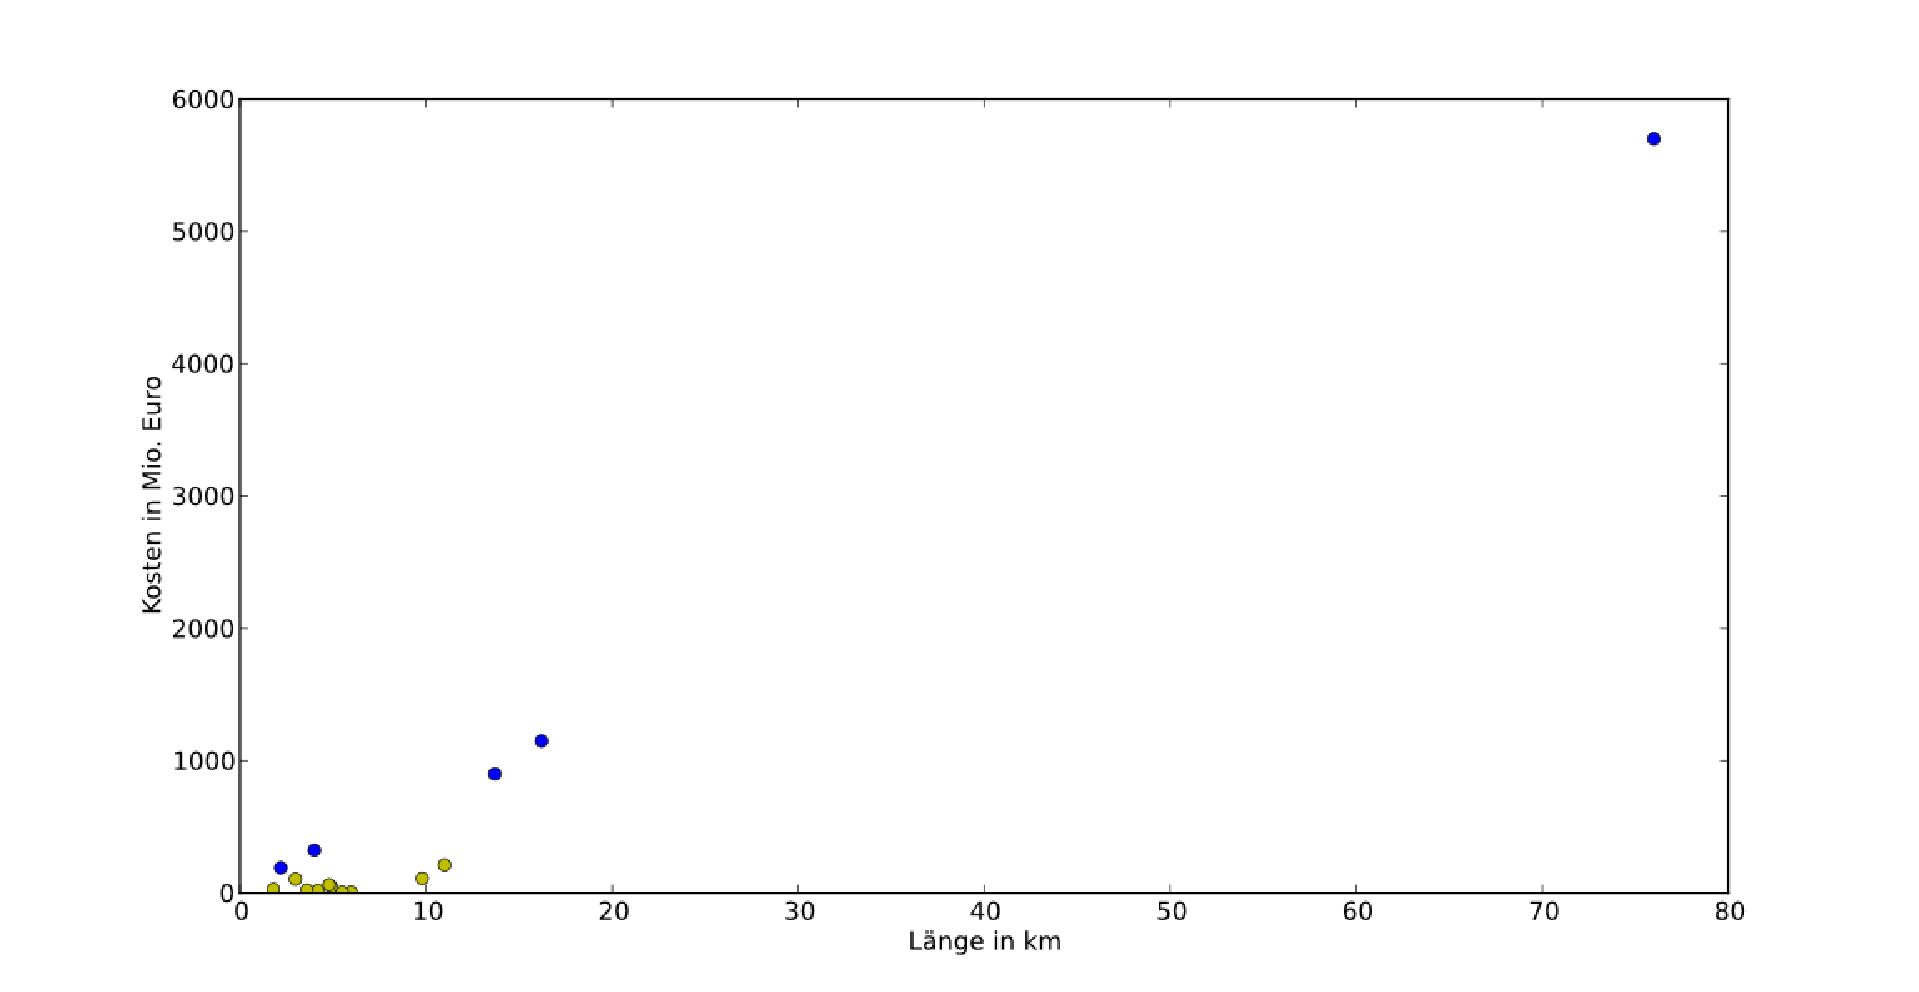
\includegraphics[width=\textwidth]{plot/overview.pdf}
\end{frame}

% ----------------------------------------------------------

\begin{frame}
  \frametitle{Erste Ergebnisse}
  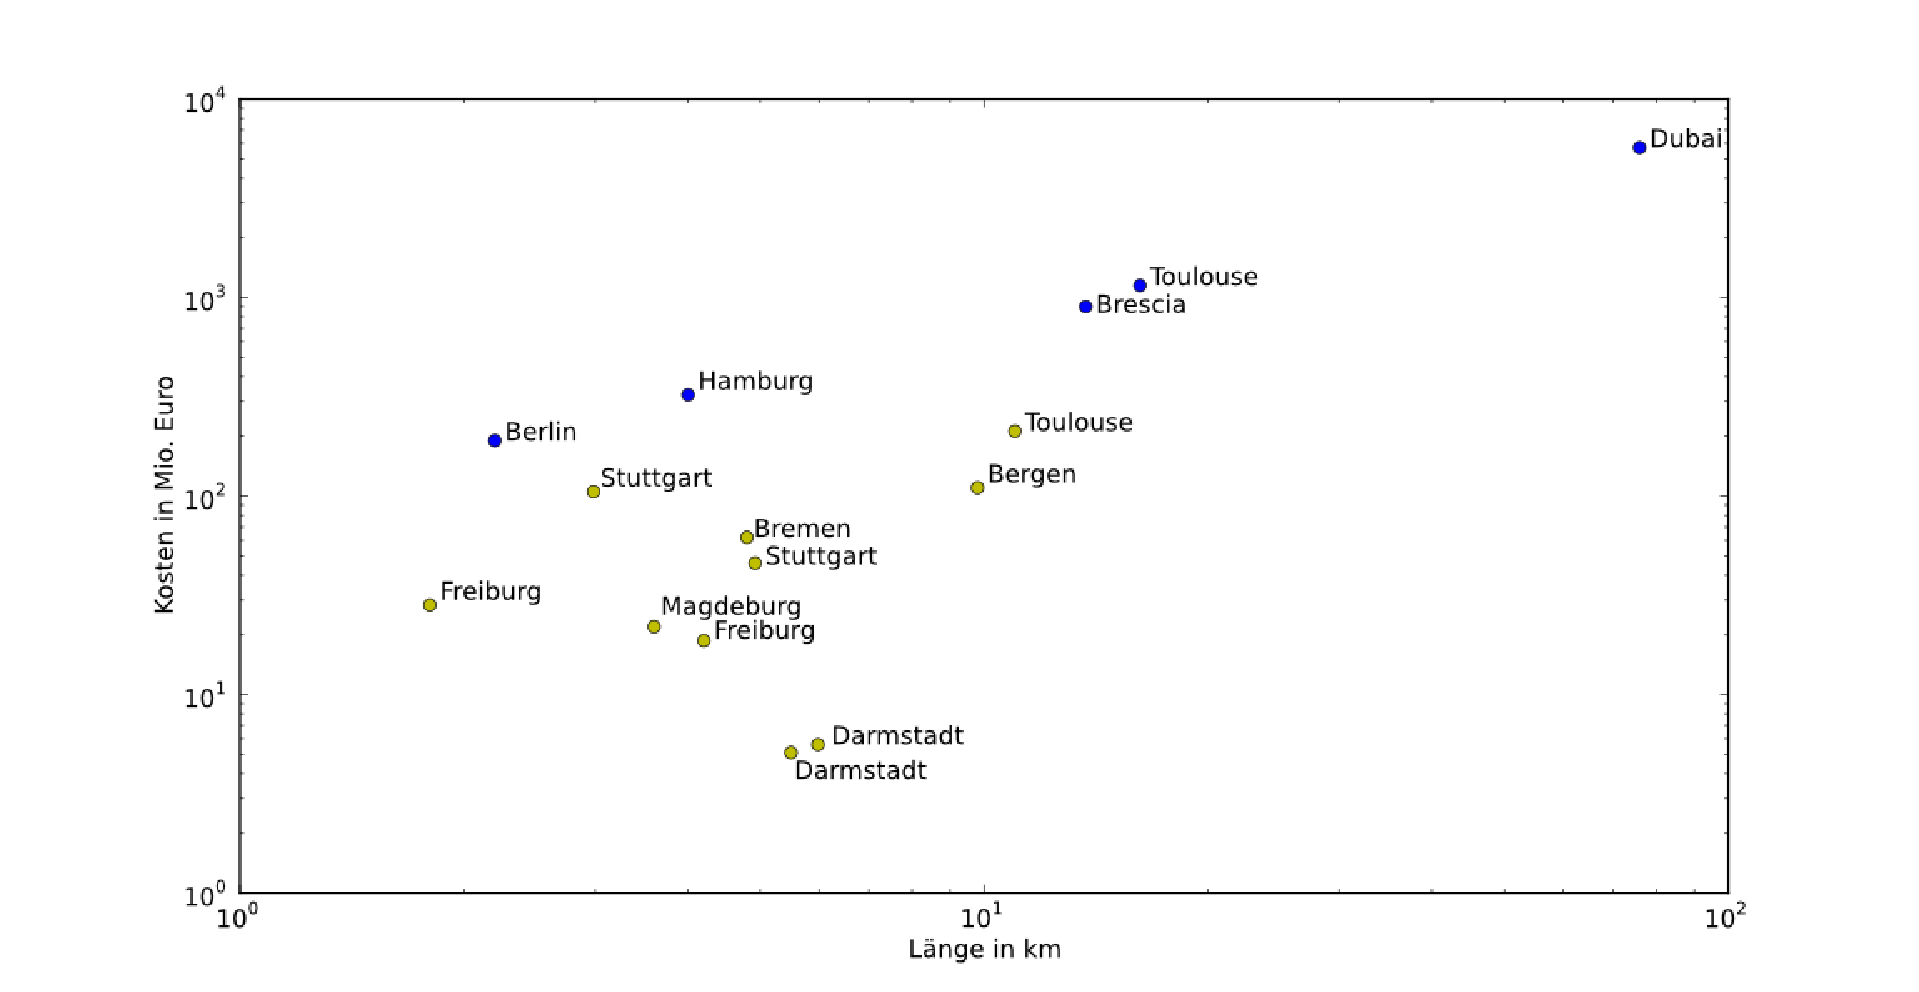
\includegraphics[width=\textwidth]{plot/detail.pdf}
\end{frame}

% ----------------------------------------------------------

\section{Quellen}
\begin{frame}[allowframebreaks]
  \frametitle{Quellen}

  \nocite{UmrechnungGoldmark}
  \nocite{buernheim1997bahnen}
  \nocite{hoeltge1992hessen}
  \nocite{BybaneBergen}
  \nocite{BergenCurrentStatus}
  \nocite{midttrafik}
  \nocite{UmrechnungKronen}
  \nocite{osm}
  \nocite{ba3reform}
  \nocite{ReformEroeffnung}
  \nocite{hallodubai}
  \nocite{gulfnews2009costs}

  \begin{scriptsize}
    \bibliography{main}
  \end{scriptsize}
\end{frame}

% ----------------------------------------------------------



\end{document}
